\documentclass{article}
\usepackage{amsmath}
\usepackage{graphicx}
\usepackage{mathtools} % for Aboxed inside align


\graphicspath{{./images/}}

\title{Unit 1}
\author{Strannik}
\date{2023 February - 2023 June}


\begin{document}
\maketitle
\section{Introduction to Vectors}
\begin{itemize}
  \item Vectors are just direction and length
  \item All parallel vectors have same unit vector.
  \item{Position Vector}
  \begin{align}
    \vec{v} = \langle x_2 - x_1, y_2 - y_1 \rangle = \langle v_1, v_2 \rangle
  \end{align}
  \item{Magnitude}
  \begin{align}
    \|\vec{v}\| = \sqrt{(v_1)^2 + (v_2)^2}
  \end{align}
  \item{Scalar}
  \begin{align}
    c\cdot\vec{v} = \langle c\cdot v_1, c\cdot v_2 \rangle
  \end{align}
  \item{Unit Vector}
  \begin{align}
    \hat{u} &= \frac{\vec{v}}{\|\vec{v}\|} \\
    \vec{v} &= \|\vec{v}\|\cdot\hat{u}
  \end{align}
  \item{Standard Basis Vectors}
  \begin{itemize}
    \item $x$-Direction: $\hat{i} = \langle 1, 0 \rangle$
    \item $y$-Direction: $\hat{j} = \langle 0, 1 \rangle$
  \end{itemize}
  \begin{align}
    \vec{v} &= v_1\cdot\hat{i} + v_2\cdot\hat{j} \\
    \hat{u} &= \cos(\theta)\cdot\hat{i} + \sin(\theta)\cdot\hat{j}
  \end{align}
\end{itemize}


\section{Vectors in 3D}
\begin{itemize}
  \item Vectors are parallel if they are scalar multiples: \(\vec{a}\parallel\vec{b} \quad\textrm{IFF}\quad \vec{a} = c\cdot\vec{b}\)
  \item Basics:
  \begin{align}
    \textrm{Distance} &= \sqrt{(x_2 - x_1)^2 + (y_2 - y_1)^2 + (z_2 - z_1)^2} \\
    \textrm{Midpoint} &= \left( \frac{x_1 + x_2}{2}, \frac{y_1 + y_2}{2}, \frac{z_1 + z_2}{2} \right) \\
  \textrm{Position Vector} &= \vec{v} = \langle v_1, v_2, v_2 \rangle = v_1\cdot\hat{i} + v_2\cdot\hat{j} + v_3\cdot\hat{k} \\
  \textrm{Magnitude} &= \|\vec{v}\| = \sqrt{(v_1)^2 + (v_2)^2 + (v_3)^2}
  \end{align}
  \item Spheres:
  \begin{itemize}
    \item Center = $(h, k, l)$
    \item Radius = $r$
  \end{itemize}
  \begin{align}
    (x - h)^2 + (y - k)^2 + (z - l)^2 = r^2
  \end{align}
\end{itemize}


\section{Dot Product}
\begin{itemize}
  \item Adds the products of corresponding components of 2 vectors
  \item Dot Product gives you a scalar
  \begin{align}
    \begin{split}
      \vec{a} &= \langle a_1, a_2, a_3 \rangle \\
      \vec{b} &= \langle b_1, b_2, b_3 \rangle \\
      \vec{a}\cdot\vec{b} &= (a_1)(b_1) + (a_2)(b_2) + (a_3)(b_3) = c \\
      \vec{v}\cdot\vec{v} &= \|\vec{v}\|^2 \\
    \end{split} \\
    \begin{split} \\
      \|\vec{v} - \vec{w}\|^2 &= \|\vec{w}\|^2 + \|\vec{v}\|^2 - 2\cdot\|\vec{w}\|\cdot\|\vec{v}\|\cdot\cos\theta \\
      \vec{v}\cdot\vec{w} &= \|\vec{v}\|\cdot\|\vec{w}\|\cdot\cos\theta \\
      \cos\theta &= \frac{\vec{v}\cdot\vec{w}}{\|\vec{v}\|\cdot\|\vec{w}\|} \\
      \theta &= \cos^{-1} \left( \frac{\vec{v}\cdot\vec{w}}{\|\vec{v}\|\cdot\|\vec{w}\|} \right) \\
    \end{split}
  \end{align}

  \item Angle between 2 vectors
  \begin{itemize}
    \item Parallel vectors
    \begin{align}
      \begin{split}
        \theta = 0 \\
        \theta = \pi
      \end{split}
    \end{align}
    \item Perpendicular (orthogonal) vectors
      \begin{align}
        \begin{split}
          \theta = \frac{\pi}{2} \\
          \vec{v}\cdot\vec{w} = 0
        \end{split}
      \end{align}
    \item Mutually Orthogonal
    \begin{align}
      \hat{i}\cdot\hat{j} = \hat{i}\cdot\hat{k} = \hat{j}\cdot\hat{k} = 0 \\
      \hat{i}\cdot\hat{i} = \hat{j}\cdot\hat{j} = \hat{k}\cdot\hat{k} = 1
    \end{align}
  \end{itemize}

  \item Vector Projection: the vector that $\vec{v}$ creates in the direction of $\vec{w}$
  \begin{align}
    \begin{split}
      \textrm{Comp}_{\vec{w}}\vec{v} &= \|\textrm{Proj}_{\vec{w}}\vec{v}\| \\
      \textrm{Comp}_{\vec{w}}\vec{v} &= \|\vec{v}\|\cdot\cos{\theta} = \frac{\vec{v}\cdot\vec{w}}{\|\vec{w}\|}
    \end{split} \\
    \Aboxed{
      \textrm{Proj}_{\vec{w}}\vec{v} &= \left( \frac{\vec{v}\cdot\vec{w}}{\|\vec{w}\|^2} \right) \cdot\vec{w}
    }
  \end{align}

  \item Work: the component of a Force ($\vec{F}$) along a directed path ($\vec{d}$)
  \begin{align}
    \begin{split}
      W &= \|\vec{F}\|\cdot\cos(\theta)\cdot\|\vec{d}\| \\
      W &= \vec{F}\cdot\vec{d}
    \end{split}
  \end{align}
\end{itemize}


\section{Direction Cosines}
  \begin{figure}[h]
    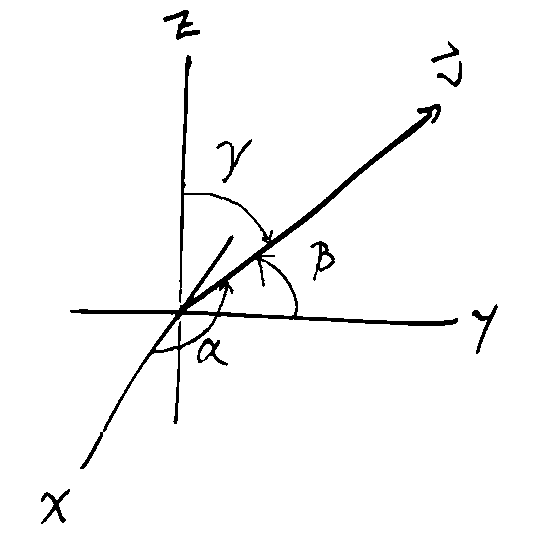
\includegraphics[scale=0.5]{direction_angles}
    \centering
    \label{fig:direction_angles}
  \end{figure}
\begin{itemize}
  \item For 3D graph imagine cones made by rotating the vector around each axis
  \item $\alpha, \beta, \gamma$ are the direction angles of $\vec{v}$
  \begin{align}
    \begin{split}
      \cos(\alpha) &= \frac{\vec{v}\cdot\hat{i}}{\|\vec{v}\|\cdot\|\hat{i}\|} = \frac{v_1}{\|\vec{v}\|} \\
      \cos(\beta) &= \frac{v_2}{\|\vec{v}\|} \\
      \cos(\gamma) &= \frac{v_3}{\|\vec{v}\|} \\
    \end{split} \\
    \begin{split}
      \cos^2(\alpha) + \cos^2(\beta) + \cos^2(\gamma) &= 1 \\
      \left( \frac{v_1}{\|\vec{v}\|} \right)^2 + \left( \frac{v_2}{\|\vec{v}\|} \right)^2 + \left( \frac{v_3}{\|\vec{v}\|} \right)^2 &= 1 \\
      \frac{(v_1)^2 + (v_2)^2 + (v_3)^2}{\|\vec{v}\|^2} &= 1 \\
    \end{split} \\
    \begin{split}
      \hat{u} = \cos(\alpha)\cdot\hat{i} + \cos(\beta)\cdot\hat{j} + \cos(\gamma)\cdot\hat{k}
    \end{split}
  \end{align}
\end{itemize}


\section{The Cross Product}
\begin{itemize}
  \item The Determinant
  \begin{align}
    \begin{vmatrix}
      a_1 & a_2 \\
      b_1 & b_2
    \end{vmatrix}
    &= a_1b_2-a_2b_1 \\
    \begin{vmatrix}
      a_1 & a_2 & a_3 \\
      b_1 & b_2 & b_3 \\
      c_1 & c_2 & c_3
    \end{vmatrix}
    &=
    \begin{vmatrix}
      b_2 & b_3 \\
      c_2 & c_3
    \end{vmatrix}
    \cdot a_1 -
    \begin{vmatrix}
      b_1 & b_3 \\
      c_1 & c_3
    \end{vmatrix}
    \cdot a_2 +
    \begin{vmatrix}
      b_1 & b_2 \\
      c_1 & c_2
    \end{vmatrix}
    \cdot a_3
  \end{align}
  \item Cross Product gives you a vector
  \begin{align}
    \Aboxed{
      \vec{a}\times\vec{b} &= (a_2b_3-a_3b_2)\hat{i} + (a_3b_1-a_1b_3)\hat{j} + (a_1b_2-a_2b_1)\hat{k}
    } \\
    \vec{a}\times\vec{b} &=
    \begin{vmatrix}
      \hat{i} & \hat{j} & \hat{k} \\
      a_1 & a_2 & a_3 \\
      b_1 & b_2 & b_3
    \end{vmatrix}
    =
    \begin{vmatrix}
      a_2 & a_3 \\
      b_2 & b_3
    \end{vmatrix}
    \cdot \hat{i} -
    \begin{vmatrix}
      a_1 & a_3 \\
      b_1 & b_3
    \end{vmatrix}
    \cdot \hat{j} +
    \begin{vmatrix}
      a_1 & a_2 \\
      b_1 & b_2
    \end{vmatrix}
    \cdot \hat{k} \label{crossproduct-by-matrix}
  \end{align}
  \begin{itemize}
    \item $\vec{a}\times\vec{b}$ gives you a vector \textbf{orthogonal} to \textbf{both} $\vec{a}$ and $\vec{b}$
    \item $\vec{b}\times\vec{a}$ gives you also a vector \textbf{orthogonal} to \textbf{both} $\vec{b}$ and $\vec{a}$
    \begin{itemize}
      \item $\vec{a}\times\vec{b} = -(\vec{b}\times\vec{a})$
    \end{itemize}
  \end{itemize}
  \item $\theta$ between $\vec{a}$ and $\vec{b}$ is always $0\leq\theta\leq\pi$
  \begin{itemize}
    \item $\sin(\theta)\geq 0$ in Cross Product
  \end{itemize}
  \item If $\vec{a}\times\vec{b} = 0$, then $\vec{b}$ and $\vec{a}$ are parallel
  \begin{align}
      \|\vec{a}\times\vec{b}\| &= \|\vec{a}\|\cdot\|\vec{b}\|\cdot\sin(\theta) \label{mag-of-cross-product} \\
    \begin{split}
      \vec{a}\times\vec{b} &= \|\vec{a}\times\vec{b}\|\cdot\hat{u} \\
      \Aboxed{
        \vec{a}\times\vec{b} &= \|\vec{a}\|\cdot\|\vec{b}\|\cdot\sin(\theta)\cdot\hat{u}
      }
    \end{split}
  \end{align}
  \begin{itemize}
    \item With a non-zero vector  $\vec{a}\times\vec{b} = 0$ only if $\sin(\theta) = 0$
    \begin{itemize}
      \item This means $\theta = 0$ or $\theta = \pi$, therefore $\vec{a}$ and $\vec{b}$ are parallel
    \end{itemize}
  \item \textbf{Don't use Cross Product to check if vectors are parallel - just check if they are scalar multiples}
  \end{itemize}
  \item Area of a parallelogram and triangle
  \begin{align}
    A_P &= \|\vec{a}\|\cdot\|\vec{b}\|\cdot\sin(\theta) = \|\vec{a}\times\vec{b}\| \\
    A_T &= \frac{1}{2}\cdot\|\vec{a}\times\vec{b}\|
  \end{align}
  \item Volume of a parallelepiped
  \begin{figure}[h]
    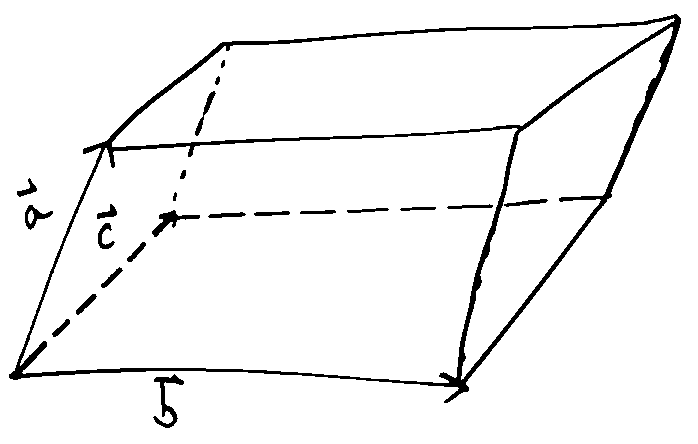
\includegraphics[scale=0.4]{parallelepiped}
    \centering
    \label{fig:parallelepiped}
  \end{figure}
  \begin{align}
    \begin{split}
      V &= \|\vec{b}\times\vec{c}\|\cdot\|\vec{a}\|\cdot\cos(\theta) \\
      \Aboxed{
        V &= |\vec{a}\cdot(\vec{b}\times\vec{c})|
      }
    \end{split}
  \end{align}
  \item Dot Product with Cross Product shortcut
  \begin{align}
    \vec{a}\cdot(\vec{b}\times\vec{c}) =
    \begin{vmatrix}
      a_1 & a_2 & a_3 \\
      b_1 & b_2 & b_3 \\
      c_1 & c_2 & c_3
    \end{vmatrix}
  \end{align}
  \begin{itemize}
    \item Use technique from equation \ref{crossproduct-by-matrix}
    \item If $\vec{a}\cdot(\vec{b}\times\vec{c}) = 0$, it means that $\vec{a}$, $\vec{b}$ and $\vec{c}$ are coplanar
  \end{itemize}
  \item $\vec{a}\times\vec{b}\perp\vec{a}$ and $\perp\vec{b}$
  \begin{itemize}
    \item $(\vec{a}\times\vec{b})\cdot\vec{a} = 0$
  \end{itemize}
  \item Torque can be represented by $\|\vec{a}\times\vec{b}\|$
  \begin{itemize}
    \item It also can be represented by $\|\vec{a}\|\cdot\|\vec{b}\|\cdot\sin(\theta)$ (see equation \ref{mag-of-cross-product})
  \item $\|\vec{\tau}\| = \|\vec{r}\|\cdot\|\vec{F}\|\cdot\sin(\theta)$
    \begin{itemize}
      \item $r = \textrm{Lever}$
      \item $F = \textrm{Force}$
    \end{itemize}
  \end{itemize}
\end{itemize}


\section{Lines and Planes in 3D}
\subsection{Lines}
\begin{itemize}
\item Line is a point and vector that gives direction
\item Any vector on the line is the same as direction vector times scalar
  \begin{itemize}
  \item $\vec{P_0P} = t\cdot\vec{v}$
  \end{itemize}
\item Parametric equations of a line in 3D
  \begin{itemize}
  \item $P_0(x_0, y_0, z_0)$
  \item $\vec{v} = \langle a, b, c \rangle$
  \end{itemize}
  \begin{align} 
    x = x_0 + at \quad y = y_0 + bt \quad z = z_0 + ct \label{line-parametric}
  \end{align}
\item Symmetric equation of a line in 3D
  \begin{align}
    \begin{split}
      t = \frac{x-x_0}{a} \quad t = \frac{y-y_0}{b} \quad t = \frac{z-z_0}{c} \\
      \Aboxed{
      \frac{x-x_0}{a} = \frac{y-y_0}{b} = \frac{z-z_0}{c}
      }
    \end{split}
  \end{align}
\item If a direction $a = 0$, then line lies in $x = x_0$ plane (parallel to $yz$-plane)
  \item Lines are $\parallel$ if their direction vectors are $\parallel$ (Scalar Multiples)
\end{itemize}

\subsection{Planes}
\begin{itemize}
\item A plane is defined by a point and a vector that is normal to this plane
\item Normal - a vector $\perp$ to a plane
\item Standard Form equation of a plane
\begin{align}
  a(x-x_0)+b(y-y_0)+c(z-z_0) = 0
\end{align}
\item General Form equation of a plane
\begin{align}
  ax+by+cz=d \label{plane-general}
\end{align}
\item The planes are $\parallel$ if normals are $\parallel$ 
\item The planes are $\perp$ if normals are $\perp$
\item Angle between planes = angle between normals
\item When given 3 points, make 2 vectors starting from one of the points and Cross Product them. This will give you a normal vector, so by using it with that starting point you can get a definition of the plane.
\item To find the point of intersection of a line with a plane plug in Parametric equations of the line (see equations \ref{line-parametric}) into Genereal Form equation of the plane (see equation \ref{plane-general})
\item To find the line of intersection of 2 planes do Cross Product of the planes' normals, the result of which will be the line's direction vector. Then set $x/y/z = 0$ in the system of plane equations and solve for the variables, which will be the line's point.
\end{itemize}

\subsection{Distances}
\begin{itemize}
  \item Distance between a plane and a point
  \begin{itemize}
    \item $P_0(x_0, y_0, z_0)$ is a point on the plane
    \item $P_1(x_1, y_1, z_1)$ is the given point not on the plane
    \item $\vec{n} = \langle a, b, c \rangle$
    \item $d = ax_0 + by_0 + cz_0$, just like in Genereal Form equation of a plane (see equation \ref{plane-general})
  \end{itemize}
  \begin{align}
    D = \textrm{Comp}_{\vec{n}}\vec{P_0P_1} = \frac{\vec{P_0P_1}\cdot\vec{n}}{\|\vec{n}\|} = \frac{|ax_1 + by_1 + cz_1 - d|}{\sqrt{a^2 + b^2 + c^2}}
  \end{align}
  
  \item Distance between 2 parallel planes
  \begin{align}
    D = \frac{|d_1 - d_2|}{\sqrt{a^2 + b^2 + c^2}} \label{planes-parallel-distance}
  \end{align}
  \begin{itemize}
    \item \textbf{Make sure the General Form equations only differ in $d$}
  \end{itemize}

  \item Distance between 2 skew lines
  \begin{itemize}
    \item Skew lines are non-parallel lines in 3D that don't intersect
    \item Skew lines can be contained by parallel planes
  \end{itemize}
  \begin{enumerate}
    \item Find the direction vectors of the lines: $\vec{v_1}$ and $\vec{v_2}$
    \item Find the common normal: $\vec{n} = \vec{v_1}\times\vec{v_2}$
    \item Create 2 General Form equation of the prarallel planes by using given points of the lines and the shared normal: $P_1$ \& $\vec{n}$ and $P_2$ \& $\vec{n}$
    \item Use equation \ref{planes-parallel-distance} to find the distance
  \end{enumerate}

  \item Distance between a line and a point
  \begin{enumerate}
    \item Starting from point on the line, make a vector to the given point: $\vec{u}$
    \item $\vec{v}$ is given from line's definition
    \item Then use equation below
  \end{enumerate}
  \begin{align}
    D = \frac{\|\vec{u}\times\vec{v}\|}{\|\vec{v}\|}
  \end{align}
\end{itemize}


\section{Cylinders and Surfaces}
\subsection{Cylinders}
\begin{figure}[h]
  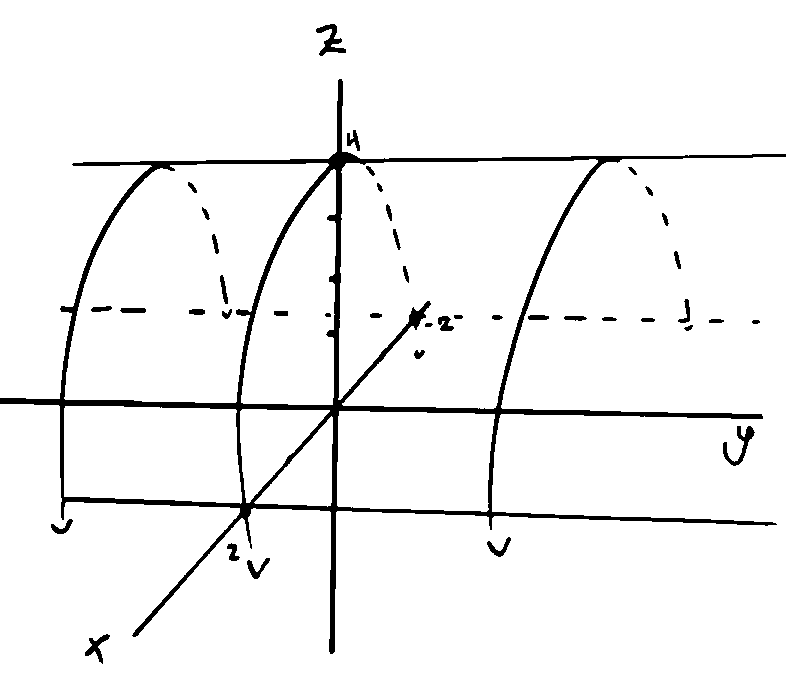
\includegraphics[scale=0.4]{cylinder-3D}
  \centering
  \caption{Example of a Cylinder: $z = 4 - x^2$}
  \label{fig:cylinder-3D}
\end{figure}
\begin{itemize}
  \item \textbf{A Cylinder doesn't have to look like a cylinder, it is just a shape that doesn't change as it goes along one of the axes}
  \item Equations only have 2 variables. They give a "trace" of the curve on the coordinate plane denoted by the given variables.
  \item The curve is directed along the axis of the missing variable in the equation
  \item The curve/trace does not change along the direction axis
\end{itemize}

\subsection{General Surfaces}
\begin{itemize}
  \item Have all 3 variables
  \item Traces occur on coordinate planes and/or on planes $\parallel$ to coordinate planes
  \item Still directed along an axis, but the trace changes along the axis
  \item Graphing steps:
  \begin{enumerate}
    \item Determine the type of surface
    \item Determine the direction axis
    \item Find trace on coordinate plane
    \item Find at least 2 other traces along the direction axis
  \end{enumerate}
\end{itemize}
\subsubsection{Elipsoids}
\begin{figure}[h]
  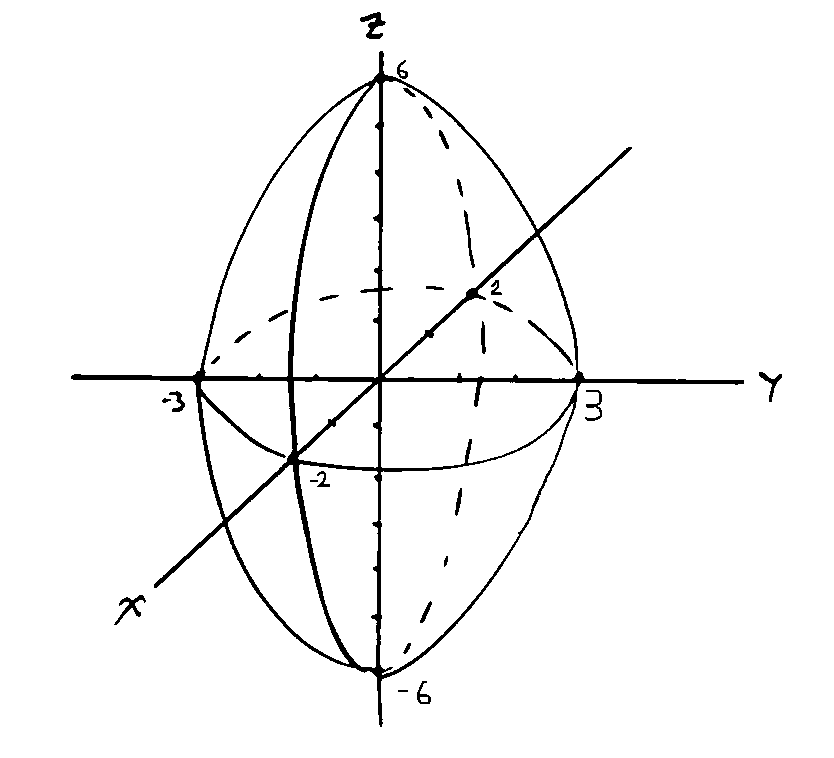
\includegraphics[scale=0.5]{elipsoid}
  \centering
  \caption{Example of an Elipsoid: $\frac{x^2}{2^2} + \frac{y^2}{3^2} + \frac{z^2}{6^2} = 1$}
  \label{fig:elipsoid}
\end{figure}
\begin{align}
  \frac{x^2}{a^2} + \frac{y^2}{b^2} + \frac{z^2}{c^2} = 1
\end{align}
\begin{itemize}
  \item How to tell if it is an Elipsoid?
  \begin{enumerate}
    \item All $(+)$
    \item All squared
    \item Has a constant
  \end{enumerate}
  \item Standard Form helps with traces
  \item Intercepts:
  \begin{align}
    \begin{split}
      x = \pm a \\
      y = \pm b \\
      z = \pm c
    \end{split}
  \end{align}
\end{itemize}
\subsubsection{1-Sheet Hyperboloids}
\begin{figure}[h]
  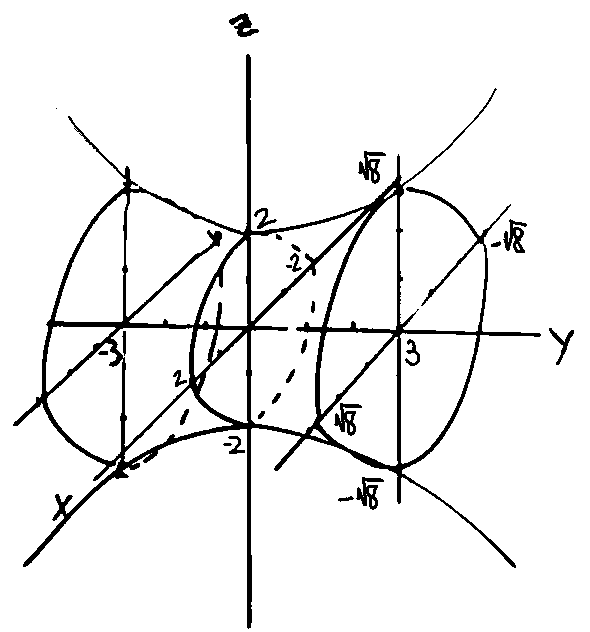
\includegraphics[scale=0.5]{1-sheet-hyperboloid}
  \centering
  \caption{Example of a 1-Sheet Hyperboloid: $\frac{x^2}{2^2} - \frac{y^2}{3^2} + \frac{z^2}{2^2} = 1$}
  \label{fig:1-sheet-hyperboloid}
\end{figure}
\begin{align}
  \frac{x^2}{a^2} + \frac{y^2}{b^2} - \frac{z^2}{c^2} = 1
\end{align}
\begin{itemize}
  \item It doesn't matter which term is negative
  \item How to tell if it is a 1-Sheet Hyperboloid?
  \begin{enumerate}
    \item Has 1 $(-)$
    \item All squared
    \item Has a constant
  \end{enumerate}
  \item Standard Form helps with traces
  \item Always is directed along the axis of $(-)$ term variable
  \item How to graph?
  \begin{enumerate}
    \item Set $(-)$ variable = 0 and $= \pm\sqrt\textrm{Denominator}$
    \item This will give you 3 traces
    \item These traces will always be circles or eliplses
  \end{enumerate}
\end{itemize}
\subsubsection{2-Sheet Hyperboloids}
\begin{figure}[h]
  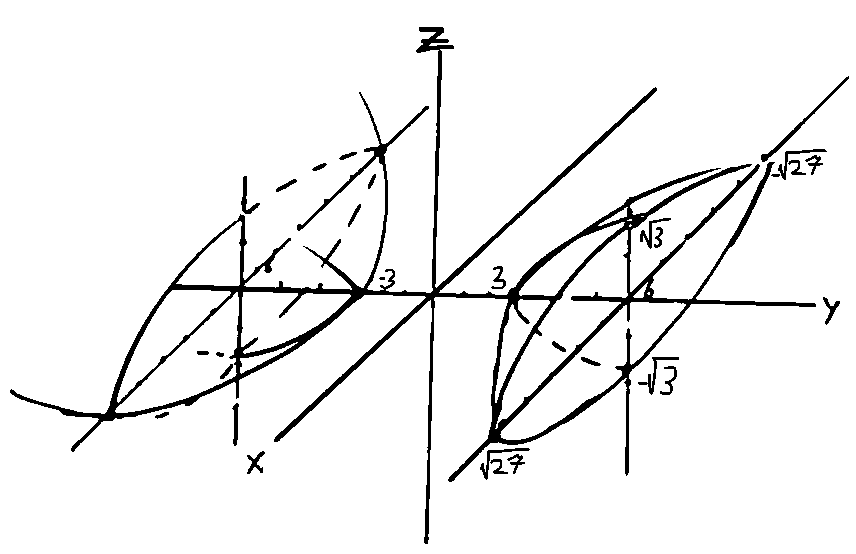
\includegraphics[scale=0.5]{2-sheet-hyperboloid}
  \centering
  \caption{Example of a 2-Sheet Hyperboloid: $-\frac{x^2}{3^2} + \frac{y^2}{3^2} - \frac{z^2}{1^2} = 1$}
  \label{fig:2-sheet-hyperboloid}
\end{figure}
\begin{align}
  -\frac{x^2}{a^2} - \frac{y^2}{b^2} + \frac{z^2}{c^2} = 1
\end{align}
\begin{itemize}
  \item It doesn't matter which term is positive
  \item How to tell if it is a 2-Sheet Hyperboloid?
  \begin{enumerate}
    \item Has 1 $(+)$
    \item All squared
    \item Has a constant
  \end{enumerate}
  \item Standard Form helps with traces
  \item Always is directed along the axis of $(+)$ term variable
  \item How to graph?
  \begin{enumerate}
    \item Setting $(+)$ variable = 0 \textbf{does nothing!}
    \item Set both $(-)$ variables = 0 to get axis intercept
    \item Set $(+)$ variable = values divisible by denominator
  \end{enumerate}
\end{itemize}
\subsubsection{Cones}
\begin{figure}[h]
  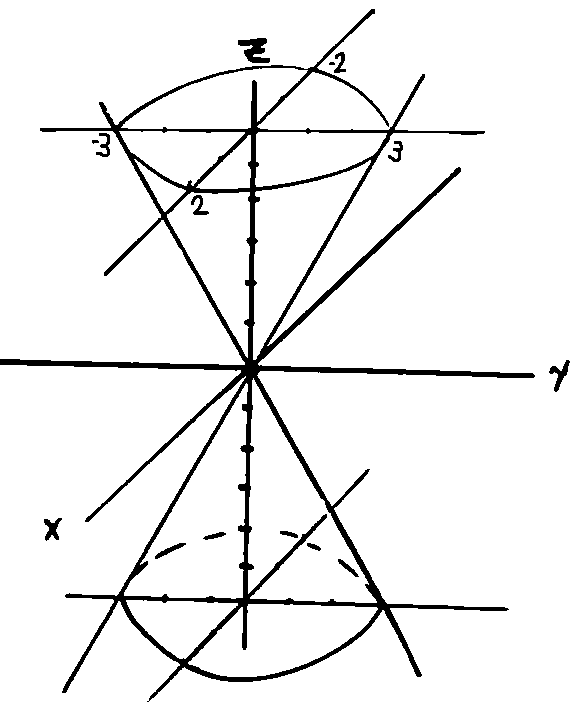
\includegraphics[scale=0.5]{cone}
  \centering
  \caption{Example of a Cone: $\frac{x^2}{2^2} + \frac{y^2}{3^2} - \frac{z^2}{6^2} = 0$}
  \label{fig:cone}
\end{figure}
\begin{align}
  \frac{x^2}{a^2} + \frac{y^2}{b^2} - \frac{z^2}{c^2} = 0
\end{align}
\begin{itemize}
  \item It doesn't matter which term is negative
  \item If you see 2 negatives, you can fix this since there is no constant on other side to change its sign when you multiply both sides by $-1$
  \item How to tell if it is a Cone?
  \begin{enumerate}
    \item Has 1 $(-)$
    \item All squared
    \item \textbf{No} constant
  \end{enumerate}
  \item Standard Form helps with traces
  \item Always is directed along the axis of $(-)$ term variable
  \item How to graph?
  \begin{enumerate}
    \item Setting $(-)$ variable = 0 \textbf{tells you nothing!} Cones always cross the origin
    \item Set $(-)$ variable = values divisible by denominator
    \item This will give you traces that are circles or elipses
  \end{enumerate}
\end{itemize}
\subsubsection{Paraboloids}
\begin{figure}[h]
  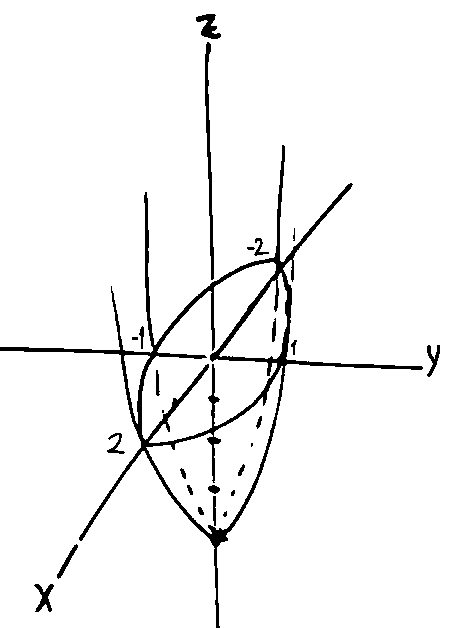
\includegraphics[scale=0.5]{paraboloid}
  \centering
  \caption{Example of a Paraboloid: $z = x^2 + 4y^2 - 4$}
  \label{fig:paraboloid}
\end{figure}
\begin{align}
  \frac{x^2}{a^2} + \frac{y^2}{b^2} = cz
\end{align}
\begin{itemize}
  \item Standard Form helps with traces only if the Paraboloid is \textbf{shifted}
  \item How to tell if it is a Paraboloid?
  \begin{enumerate}
    \item 3 variables with 2 of them squared
    \item Squared variables are $(+)$
  \end{enumerate}
  \item Opens along the axis of variable with degree of 1
  \item Coefficient of degree 1 variable gives direction
  \item How to graph?
  \begin{enumerate}
    \item Set degree 1 variable = 0 to get a trace on a coordinate plane (Works only if the Paraboloid is shifted)
    \item If it is not shifted, just pick a value further in the direction of the Paraboloid to get the trace
    \item 1 trace is enough
  \end{enumerate}
\end{itemize}
\subsubsection{Hyperbolic Paraboloids}
\begin{figure}[h]
  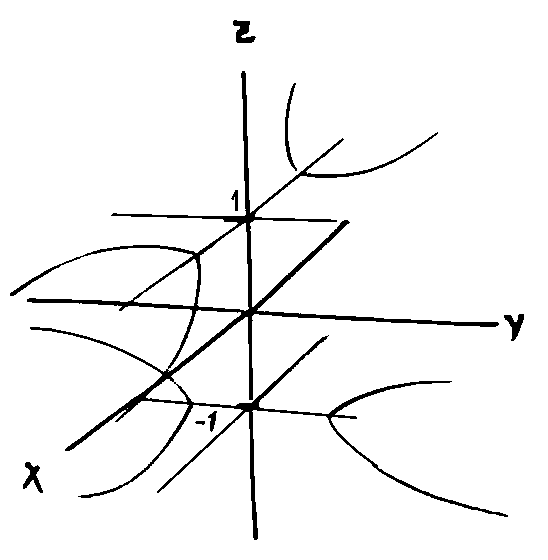
\includegraphics[scale=0.5]{hyperbolic-paraboloid}
  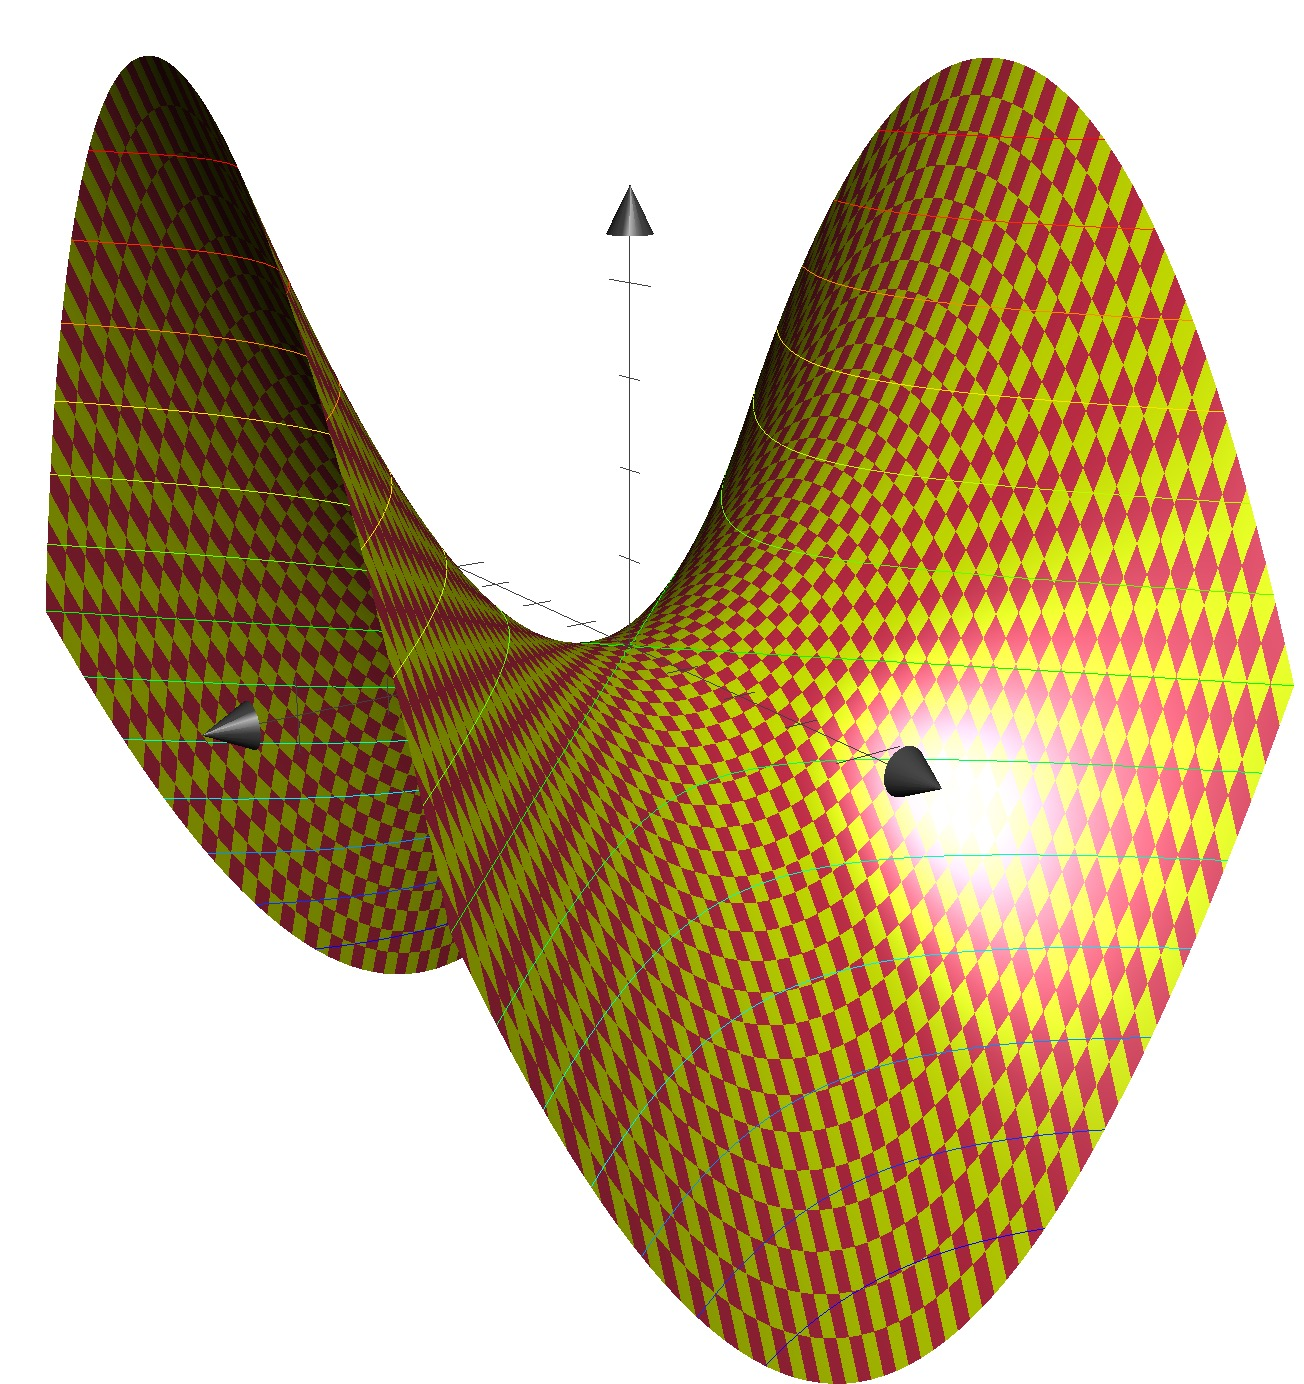
\includegraphics[scale=0.1]{hyperbolic-paraboloid-digital}
  \centering
  \caption{Example of a Hyperbolic Paraboloid: $x^2 - y^2 = z$}
  \label{fig:hyperbolic-paraboloid}
\end{figure}
\begin{align}
  \frac{x^2}{a^2} - \frac{y^2}{b^2} = cz
\end{align}
\begin{itemize}
  \item Standard Form doesn't help you with traces
  \item How to tell if it is a Hyperbolc Paraboloid?
  \begin{enumerate}
    \item 3 variables with 2 of them squared
    \item One of the terms with squared variables is $(-)$ (it doesn't matter which one)
  \end{enumerate}
  \item How to graph?
  \begin{enumerate}
    \item Degree 1 variable gives direction axis
    \item Plug in $(+)$ and $(-)$ numbers to degree 1 variable
  \end{enumerate}
\end{itemize}


\section{Cylindrical \& Spherical Coordinate Systems}
\begin{itemize}
  \item Cylindrical: 
  \begin{itemize}
    \item Polar coordinate system with $z$ component
    \item Cyl $(r, \theta, z)$
    \item Cylindrical to Rectangular:
    \begin{align}
      \begin{split}
        x &= r\cos(\theta) \\
        y &= r\sin(\theta) \\
        z &= z
      \end{split} \label{cylindrical-xyz-equations}
    \end{align}
    \item Rectangular to Cylindrical:
    \begin{align}
      \begin{split}
        r^2 = x^2 + y^2 \\
        \tan(\theta) = \frac{y}{x} \\
        z = z
      \end{split}
    \end{align}
    \item \textbf{$r$ is not the distance from origin to a point}
    \item \textbf{Must mathch quadrants and octants}
  \end{itemize}
  \item Spherical:
    \begin{itemize}
      \item Sph $(\rho, \theta, \phi)$
      \item Uses distance from origin to point $\rho$ (radius)
      \item $\theta$, just like Cyl
      \item $\phi$, angle from $(+)$ $z$-axis
      \begin{align}
        \rho\geq 0 \qquad 0\leq\theta\leq 2\pi \qquad 0\leq\phi\leq\pi
      \end{align}
      \item Spherical to Rectangular:
      \begin{align}
        r = \rho\sin(\phi) \label{spherical-r-equation}
      \end{align}
      \begin{itemize}
        \item Plug in equation \ref{spherical-r-equation} into $x$ and $y$ equations \ref{cylindrical-xyz-equations}:
      \end{itemize}
      \begin{align}
        \begin{split}
          x &= \rho\sin(\phi)\cos(\theta) \\
          y &= \rho\sin(\phi)\sin(\theta)
        \end{split} \\
        z &= \rho\cos(\phi)
      \end{align}
      \item Rectangular to Spherical:
      \begin{align}
        \begin{split}
          \rho^2 = x^2 + y^2 + z^2 \\
          \tan(\theta) = \frac{y}{x} \\
          \cos(\phi) = \frac{z}{\rho}
        \end{split}
      \end{align}
    \end{itemize}
  \item When the graph's shape isn't obvious, convert the equation to Rectangular
\end{itemize}
\end{document}
